%! TeX root = /Users/trustinnguyen/Downloads/Berkeley/Compsci/CS170/Homework/CS170Hw11/CS170Hw11.tex

\documentclass{article}
\usepackage{/Users/trustinnguyen/.mystyle/math/packages/mypackages}
\usepackage{/Users/trustinnguyen/.mystyle/math/commands/mycommands}
\usepackage{/Users/trustinnguyen/.mystyle/math/environments/article}
\graphicspath{{./figures/}}

\title{CS170Hw11}
\author{Trustin Nguyen}

\begin{document}

    \maketitle

\reversemarginpar

\section*{Study Group}
\hrule

\newpage
\section*{Decision vs Search vs Optimization}
\hrule

Recall that a vertex cover is a set of vertices in a graph such that every edge is adjacent to at least one vertex in this set.

The following are three formulations of the VERTEX COVER problem:
    \begin{itemize}
        \item As a \textit{decision problem}: Given a graph $G$, return TRUE if it has a vertex cover of size at most $b$, and FALSE otherwise.

        \item As a \textit{search problem}: Given a graph $G$, find a vertex cover of size at most $b$ (that is, return the actual vertices), or report that none exists.

        \item As an \textit{optimization problem}: Given a graph $G$, find a minimum vertex cover.
    \end{itemize}

At first glance, it may seem that search should be harder than decision, and that optimization should be even harder. We will show that if any one can be solved in polynomial time, so can the others.
    \begin{itemize}
        \item [(a)] Suppose you are handed a black box that solves VERTEX COVER (DECISION) in polynomial time. Give an algorithm that solves VERTEX COVER (SEARCH) in polynomial time.
            \begin{answer}
                The vertex cover problem is in correspondence to $2$-SAT. If an edge $(u, v)$ is in the graph, we add the clause $(u \lor v)$ to the chain of clauses. Then the problem reduces to finding $b$ vertices $v_{1}, v_{2}, \ldots, v_{b}$ such that setting the $v_{1}, \ldots, v_{b}$ to true satisfies all clauses. 

                This gives a natural way of solving the problem. We pick an edge of the graph. Say that this edge is $(u^{\prime}, v^{\prime})$. Pick one vertex of that edge at random, lets say $v^{\prime}$. We remove that vertex and all its adjacent edges (this corresponds to the fact that all clauses containing $v^{\prime}$ will be satisfied if $v^{\prime} = True$). 

                Now we run VERTEX COVER(DECISION) on the remaining graph with $b - 1$. If it returns true, we know that $v^{\prime}$ is in a vertex cover, otherwise, we say that $u^{\prime}$ is in our vertex cover. Repeat until we have no more clauses in our $2$-SAT. The vertices we have chosen will make up the vertex cover of size at most $b$.
            \end{answer}

        \item [(b)] Similarly, suppose you are handed a black box that solves VERTEX COVER (SEARCH) in polynomial time. Give an algorithm that solves VERTEX COVER (OPTIMIZATION) in polynomial time.
            \begin{answer}
                We can start with $b = 0$ and run the search algorithm, increasing $b$ by $1$ every time until the VERTEX COVER(SEARCH) reports that a vertex cover of size at most $b$ exists. The first instance will be the minimum vertex cover. A speed up would be binary searching.
            \end{answer}
    \end{itemize}

\newpage
\section*{Some Sums}
\hrule

Given an array $A = [a_{1}, a_{2}, \ldots, a_{n}]$ of non negative integers, consider the following problems:
    \begin{itemize}
        \item [1] \textbf{Partition}: Determine whether there is a subset $S \subseteq [n]$ ($[n] := \{1, 2, \ldots, n\}$) such that $\sum_{i \in S} a_{i} = \sum_{j \in ([n] \backslash S)}a_{j}$. In other words, determine whether there is a way to partition $A$ into two disjoint subsets such that the sum of the elements in each subset are equal.

        \item [2] \textbf{Subset Sum}: Given some integer $x$, determine whether there is a subset $S \subseteq [n]$ such that $\sum_{i \in S} a_{i} = x$. In other words, determine whether there is a subset of $A$ such that the sum of its elements is $x$.

        \item [3] \textbf{Knapsack}: Given some set of items each with weight $w_{i}$ and value $v_{i}$, and fixed numbers $W$ and $V$, determine whether there is some subset $S \subseteq [n]$ such that $\sum_{i \in S} w_{i} \leq W$ and $\sum_{i \in S} v_{i} \geq V$.
    \end{itemize}

For each of the following clearly describe your reduction and justify its correctness.
    \begin{itemize}
        \item [(a)] Find a linear time reduction from SUBSET SUM to PARTITION.
            \begin{answer}
                To turn our subset sum to a partition problem, consider the operation of adding the element $2x - \sum_{i} a_{i}$ to our set $A$ to get $A^{\prime}$, and calling 
                    \begin{equation*}
                        PARTITION(A^{\prime})
                    \end{equation*}
                The claim is that the truth value of $SUBSET\_SUM(A, x)$ is the same as the truth value of $PARTITION(A^{\prime})$.
                    \begin{itemize}
                        \item Suppose that we have a valid partition of $A^{\prime}$. Then we split $A^{\prime}$ into sets $L, R$ such that $\sum L = \sum R$. We know that $2x - \sum_{i} a_{i}$ can only be in one of $L$ or $R$. Wlog, say it is not in $L$. This means that
                            \begin{equation*}
                                L \subseteq A
                            \end{equation*}
                        But 
                            \begin{equation*}
                                \sum L = \frac{1}{2} \cdot \sum A^{\prime} = \sum A + 2x - \sum_{i} a_{i} = \dfrac{1}{2} \cdot 2x = x
                            \end{equation*}
                        so we have found a subset of $A$ that adds to $x$.

                        \item Suppose there is a subset of $A$ that adds to $x$. We will show that there is a partition of $A^{\prime}$. Let that subset be called $L  \subseteq A $. Then we know that:
                            \begin{equation*}
                                \sum L = x
                            \end{equation*}
                        and 
                            \begin{equation*}
                                \sum A^{\prime} \backslash L = x
                            \end{equation*}
                        as $\sum A^{\prime} = 2x$. So there is a partition of $A^{\prime}$.
                    \end{itemize}
            \end{answer}

        \item [(b)] Find a linear time reduction from SUBSET SUM to KNAPSACK.
            \begin{answer}
                Let $W = V = x$. For each item, let $w_{i} = v_{i} = a_{i}$. Then the claim is that 
                    \begin{equation*}
                        KNAPSACK(W, V, \{w\}_{i}, \{v\}_{i}) = KNAPSACK(x, x, A, A)
                    \end{equation*}
                is the same as $SUBSET\_SUM(A, x)$.
                    \begin{itemize}
                        \item Suppose that we have determined the value of $KNAPSACK(x, x, A, A)$ to be true. Then we know there is some subset $S \subseteq [n]$ such that
                            \begin{equation*}
                                \sum_{i \in S} a_{i} \geq x
                            \end{equation*}
                        and
                            \begin{equation*}
                                \sum_{i \in S} a_{i} \leq x 
                            \end{equation*}
                        so
                            \begin{equation*}
                                \sum_{i \in S} a_{i} = x
                            \end{equation*}

                        \item Suppose that we have determined the value of $SUBSET\_SUM(A, x)$ to be true. Then we know there is a subset:
                            \begin{equation*}
                                \sum_{i \in S} a_{i} = x 
                            \end{equation*}
                        so it follows
                            \begin{equation*}
                                \sum_{i \in S} a_{i} \geq x
                            \end{equation*}
                        and
                            \begin{equation*}
                                \sum_{i \in S} a_{i} \leq x 
           l                \end{equation*}
                        so $KNAPSACK(x, x, A, A)$ is true  as well.
                    \end{itemize}
            \end{answer}
    \end{itemize}

\newpage
\section*{Reduction to 3-Coloring}
\hrule

Given a graph $G = (V, E)$, a valid $3$-coloring assigns each vertex in the graph a color from $\{\text{red, green, blue}\}$ such that for any edge $(u, v)$, $u$ and $v$ have different colors. In the $3$-coloring problem, our goal is to find a valid $3$-coloring if one exists. In this problem, we will give a reduction from $3$-SAT to the $3$-coloring problem. Since we know that $3$-SAT is NP-Hard (there is a reduction to $3$-SAT from every NP problem), this will show that $3$-coloring is NP-Hard (there is a reduction to $3$-coloring from every NP problem).

In our reduction, the graph will start with three special vertices, labeled $v_{TRUE}$, $v_{FALSE}$, and $v_{BASE}$, as well as the edges $(v_{TRUE}, v_{FALSE})$, $(v_{TRUE}, v_{BASE})$, and $(v_{FALSE}, v_{BASE})$.
    \begin{itemize}
        \item [(a)] For each variable $x_{i}$ in a $3$-SAT formula, we will create a pair of vertices labeled $x_{i}$ and $\lnot x_{i}$. How should we add edges to the graph such that in any valid $3$-coloring, one of $x_{i}$, $\lnot x_{i}$ is assigned the same color as $v_{TRUE}$ and the other is assigned the same color as $v_{FALSE}$?
            \begin{answer}
                For each pairing $x_{i}, \lnot x_{i}$, create a vertex $y_{i}$ and assign it the color $v_{BASE}$. Now add edges so that the three vertices $x_{i}, \lnot x_{i}, y_{i}$ form a triangle. This ensures that either $x_{i}$ or $\lnot x_{i}$ is assigned the color $v_{TRUE}$ and the other is assigned the color $v_{FALSE}$.
            \end{answer}

        \item [(b)] Consider the following graph, which we will call a ``gadget'':
            \begin{center}
                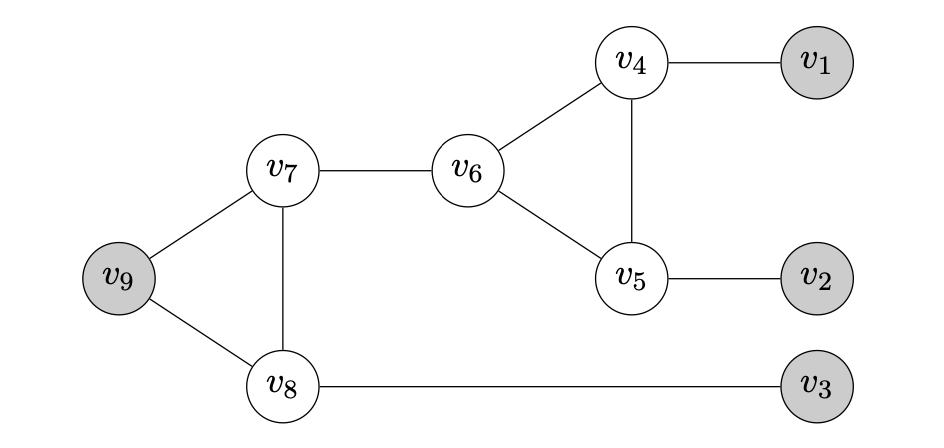
\includegraphics[scale=0.5]{graph.png}
            \end{center}
        Consider any valid $3$-coloring of this graph that does \textit{not} assign the color red to any of the gray vertices $(v_{1}, v_{2}, v_{3}, v_{9})$. Show that if $v_{9}$ is assigned the color blue, then at least one of $\{v_{1}, v_{2}, v_{3}\}$ is assigned the color blue.
            \begin{answer}
                We will prove the contrapositive. If $v_{1}, v_{2}, v_{3}$ are all non blue, then they must be some other color green. We know then the $v_{4}, v_{5}$ are non green, so $v_{6}$ must be green. Now $v_{7}, v_{8}$ are non green so $v_{9}$ must be green. So $v_{9}$ is non blue.
            \end{answer}

        \item [(c)] We have now observed the following about the graph we are creating in the reduction:
            \begin{itemize}
                \item [(i)] For any vertex, if we have the edges $(u, v_{FALSE})$ and $(u, v_{BASE})$ in the graph, then in any valid $3$-coloring $u$ will be assigned the same color as $v_{TRUE}$

                \item [(ii)] Through brute force one can also show that in a gadget, if all the following hold:
                    \begin{itemize}
                        \item [(1)] All gray vertices are assigned the color green or blue.

                        \item [(2)] $v_{9}$ is assigned the color blue.

                        \item [(3)] At least one of $\{v_{1} ,v_{2}, v_{3}\}$ is assigned the color blue.
                    \end{itemize}
                Then there is a valid coloring for the white vertices in the gadget.
            \end{itemize}
            Using these observations and your answers to the previous parts, give a reduction from $3$-SAT to $3$ coloring. Prove that your reduction is correct (you do not need to prove any of the observations above).
                \begin{answer}
                    To solve this, for every variable $x_{i}$ in our $3-SAT$, start constructing the graph by adding components of the form:
                        \begin{center}
                            \begin{fixedfigure}
                                \incfig{3satComp}
                            \end{fixedfigure}
                        \end{center}
                    where the third node is fixed at some color (gray) other than red and blue. Now for each clause in our $3-SAT$, lets say $(a_{1} \lor a_{2} \lor a_{3})$ add a gadget:
                        \begin{center}
                            \begin{fixedfigure}
                                \incfig{gadget}
                            \end{fixedfigure}
                        \end{center}
                    with the left most node fixed at color blue, and impose that the right nodes are either red or blue (not gray). Connect the rightmost nodes to their negation nodes in the triangle components that we made earlier. For example:
                        \begin{center}
                            \begin{fixedfigure}
                                \incfig{gadget3Comp}
                            \end{fixedfigure}
                        \end{center}
                    Now we claim that solving for a valid coloring of the graph is equivalent to solving the $3-SAT$.

                    We have described a way to get from $3$-SAT to $3$-coloring, and now to show that a solution on the $3$-coloring gives a solution on the $3$-SAT.
                        \begin{itemize}
                            \item Suppose there is a valid $3$-coloring of the graph. Then for every gadget, the $v_{9}$ node is blue and one of the $v_{1}, v_{2}, v_{3}$ nodes are blue also. Then this defines a correspondence to the truth value of a clause.

                            So if we have a valid $3$-coloring, the $3$-SAT is satisfied:
                                \begin{itemize}
                                    \item [1] Each clause is colored blue (Represents that the clause is evaluated to true)

                                    \item [2] One of the three nodes $v_{1}, v_{2}, v_{3}$ are true in each gadget (Represents that at least one literal in the clause is true)

                                    \item [3] None of the pairs $a_{i}, \lnot a_{i}$ are the same color (Recall we connected each $v_{1}, v_{2}, v_{3}$ in the gadget to its negation, so they cannot be the same color).
                                \end{itemize}

                            \item Now suppose that we are given a $3$-SAT that evaluates to true and the truth values of each literal. We need to show that the corresponding graph we constructed has a valid $3$-coloring.

                            Assign the color red to mean the truth value of false and blue to represent true. By the brute force observation, all gadgets have a valid coloring. We also know that none of the pairs $a_{i}, \lnot a_{i}$ are the same color. This means there is a valid coloring on every $3$ component:
                            \begin{center}
                                \begin{fixedfigure}
                                    \incfig{3satComp}
                                \end{fixedfigure}
                            \end{center}
                            Finally, there is a valid coloring on the union of the gadget graph and $3$ component graph because $x_{i}$ and $\lnot x_{i}$ are different colors (same reason).
                        \end{itemize}
                    This concludes the proof.
                \end{answer}
    \end{itemize}


\end{document}
